\subsubsection{UC\theuccount-GP - Producer Redmine invia messaggio al Gestore Personale}
    \begin{figure}[H]
		\centering
		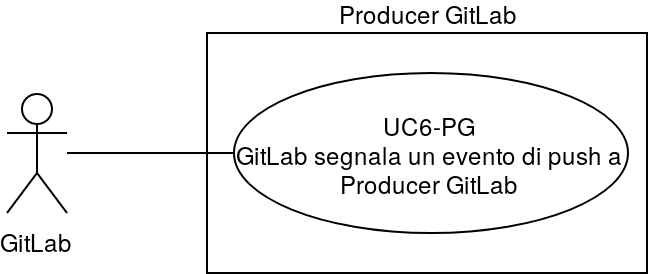
\includegraphics[width=0.8\textwidth]{img/casi_d'uso/UC6.png}\\
		\caption{UC\theuccount-GP - Producer Redmine invia messaggio al Gestore Personale}
	\end{figure}
	\begin{itemize}
		\item \textbf{Codice}: UC\theuccount-GP.
		\item \textbf{Titolo}: Producer Redmine invia messaggio al Gestore Personale.
		\item \textbf{Attori Pimari}: Producer Redmine.
		\item \textbf{Descrizione}: il Producer Redmine, dopo aver ricevuto una
		 segnalazione da Redmine, elabora il messaggio e lo invia al Gestore Personale.
		 Il messaggio finale, una volta terminata l'elaborazione, conterrà i campi:
		 \begin{itemize}
		 	\item Poject
		 	\item Topic
		 	\item Subject e opzionalmente:
		 	\begin{itemize}
		 		\item Description
		 	\end{itemize}
		 \end{itemize}
	 	Il messaggio non può contenere campi errati o mancanti per il corretto funzionamenti di \progetto, perché i campi selezionati sono obbligatori per l'apertura di una issue su Redmine.
		\item \textbf{Pecondizione}: il Producer Redmine ha ricevuto una segnalazione da Redmine.
		\item \textbf{Postcondizione}: il Producer Redmine ha elaborato e inviato al Gestore Personale il messaggio.
		\item \textbf{Scenario GPincipale}: 
		\begin{enumerate}
			\item Il Producer Redmine riceve la segnalazione di issue da Redmine
			\item Il Producer Redmine prepara il messaggio di issue in modo che venga inserito correttamente nel Gestore Personale
			\item Il Producer Redmine invia il messaggio di issue al Gestore Personale
		\end{enumerate}
		
	\end{itemize}
	
	\stepcounter{subuccount}
	\subsubsection{UC\theuccount.\thesubuccount-GP - Producer Redmine invia messaggio di apertura issue al Gestore Personale}
	
	\begin{itemize}
		\item \textbf{Codice}: UC\theuccount.\thesubuccount-GP.
		\item \textbf{Titolo}: Producer Redmine invia messaggio di apertura issue al Gestore Personale.
		\item \textbf{Attori Pimari}: Producer Redmine.
		\item \textbf{Descrizione}: il Producer Redmine, dopo aver
		ricevuto una segnalazione di apertura issue da Redmine, elabora il messaggio e lo invia al Gestore Personale.
		Il messaggio finale, una volta terminata l'elaborazione, conterrà i campi:
		\begin{itemize}
			\item Poject
			\item Topic
			\item Subject e opzionalmente:
			\begin{itemize}
				\item Description
			\end{itemize}
		\end{itemize}
		\item \textbf{Pecondizione}: il Poducer Redmine ha ricevuto una segnalazione da Redmine.
		\item \textbf{Postcondizione}: il Poducer Redmine ha elaborato e inviato al Gestore Personale il messaggio di apertura issue.

		\item \textbf{Scenario Pincipale}: 
		\begin{enumerate}
			\item Il Producer Redmine riceve la segnalazione di apertura issue da Redmine
			\item Il Producer Redmine prepara il messaggio in modo che venga inserito correttamente nel Gestore Personale
			\item Il Producer Redmine invia il messaggio di
			apertura issue al Gestore Personale
		\end{enumerate}
		
	\end{itemize}
	
	\stepcounter{subuccount}
	\subsubsection{UC\theuccount.\thesubuccount-GP - Producer Redmine invia messaggio di modifica issue al Gestore Personale}
		
		\begin{itemize}
			\item \textbf{Codice}: UC\theuccount.\thesubuccount-GP.
			\item \textbf{Titolo}: Producer Redmine invia messaggio di modifica issue al Gestore Personale
			\item \textbf{Attori Pimari}: Producer Redmine.
			\item \textbf{Descrizione}: il Producer Redmine, dopo aver
			ricevuto una segnalazione di modifica issue da Redmine, elabora il messaggio e lo invia al Gestore Personale.
			Il messaggio finale, una volta terminata l'elaborazione, conterrà i campi:
			\begin{itemize}
				\item Poject
				\item Topic
				\item Subject e opzionalmente:
				\begin{itemize}
					\item Description
				\end{itemize}
			\end{itemize}
			\item \textbf{Pecondizione}: il Producer Redmine ha ricevuto una segnalazione da Redmine.
			\item \textbf{Postcondizione}: il Producer Redmine ha elaborato e inviato al Gestore Personale il messaggio di modifica issue.
			\item \textbf{Scenario Pincipale}: 
			\begin{enumerate}
				\item Il Producer Redmine riceve la segnalazione di modifica issue da Redmine
				\item Il Producer Redmine prepara il messaggio in modo che venga inserito correttamente nel Gestore Personale
				\item Il Producer Redmine invia il messaggio di
				modifica issue al Gestore Personale
			\end{enumerate}
			\item \textbf{Estensioni}: 
			\begin{enumerate}
				\item Se ci sono dei messaggi non validi, questi vengono scartati [UC\theuccount.3-GP].
			\end{enumerate}
		\end{itemize}
	
	\stepcounter{subuccount}
	\subsubsection{UC\theuccount.\thesubuccount-GP - Producer Redmine scarta i messaggi non validi}
	
	\begin{itemize}
		\item \textbf{Codice}: UC\theuccount.\thesubuccount-GP.
		\item \textbf{Titolo}: Producer Redmine scarta i messaggi non validi.
		\item \textbf{Attori primari}: Producer Redmine.
		\item \textbf{Descrizione}: il Producer Redmine, dopo aver ricevuto una segnalazione di una modifica issue da Redmine, controlla
		se è stato modificato il campo Subject o Assignee. In caso negativo, il messaggio viene scartato.
		\item \textbf{Precondizione}: il Producer Redmine ha ricevuto una segnalazione da GitLab.
		\item \textbf{Postcondizione}: il Producer Redmine ha scartato il messaggio.
		\item \textbf{Scenario principale}: 
		\begin{enumerate}
			\item Il Producer Redmine riceve la segnalazione di modifica issue da Redmine
			\item Il Producer Redmine vede che non è stato modificato il campo Subject
			\item Il Producer Redmine scarta il messaggio non valido.
		\end{enumerate}
	\end{itemize}